\section{Preliminary Results}
\label{sec:results}
In this section, we examine preliminary results of two case-studies implemented in DFiant: an Advanced Encryption Standard~\cite{pub2001197} (AES) cipher block and an IEEE-754~\cite{IEEE2008} double-precision floating point (FP) multiplier. We compare both test cases against traditional designs, and demonstrate competing performance while simplifying code verbosity significantly. 

\subsection{Methodology}
We implemented both test cases in DFiant, constrained them by a variance of minimum frequency requirements, and compiled them to RTL. The DFiant compiler automatically pipelined the design to achieve the required minimum frequency, and generated an RTL verilog file, and an TCL constraints file. For a baseline, we obtained equivalent open-source RTL cores and Vivado HLS implementations, where possible. We disabled DFiant's support for pipelined valid/ready signaling and a blocking back-pressure, since the RTL cores did not support this capability.

We chose the following comparison metrics: the maximum clock frequency, clock cycle latency, utilizations of both look-up tables (LUTs) and flip-flop registers (FFs), and lines of code (LoC). We used Xilinx Vivado to synthesize and implement the RTL design for a Virtex-7 FPGA, part number: xc7vx485tffg1761-2. The tool was configured to use default strategy for both synthesis and implementation processes. For each design, we recorded the maximum clock frequency, LUTs, and FFs. We recorded the design latency as reported by the DFiant and Vivado HLS compilers, and the RTL cores documentation. Finally, we automatically counted the LoC \cite{danial2009cloc}, applied standard score normalization (0-100) to all metrics, and assured higher values indicate better score for all metrics. Mean score of all metrics is presented as well.

\subsection{Case Study: AES Cypher}
For baseline comparison, we used three AES cypher RTL designs from opencores.org: Das core \cite{das2010fully}, Hsing core \cite{hsing2013aes} and Salah core \cite{salah2013aespipe}. Additionally, we obtained a Vivado C++ HLS design~\cite{oflynn2014rapid}. All these designs are fully pipelined, meaning that in every cycle the design accepts new key and data inputs, and emits an encrypted data output, delayed by a fixed design latency.

%All three cores are target device agnostic
%Added metric: number of supported key sizes.
%discuss SBOX

We compiled the DFiant and Vivado HLS designs with three target clock frequencies: 200 MHz, 300 MHz, and 450 MHz. We named the designs accordingly (e.g., DFiant\_200 is the 200MHz target design). We collected the results in Table~\ref{tbl:AES_Compare_Table}, and displayed their normalized standard score in Fig.~\ref{fig:AES_Compare_Graph}. We added the supported key types quantity as a metric, since some designs support 128bit keys and do not include 192bit and 256bit keys as well. The table also includes an 'SBox BRAM Use' column, since some designs do not use memory to implement the AES SBox function.

\begin{table*}[t!]
  \centering
	\setlength\tabcolsep{2pt}
	\scriptsize
  \begin{minipage}[t][6.5cm][t]{0.8\linewidth}
    \centering
    \captionof{table}{AES Cypher RTL Designs Comparison\\(the numbering on the left associates configurations with \fig{fig:AES_Compare_Graph})}
    \label{tbl:AES_Compare_Table}
    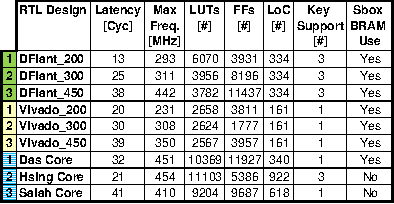
\includegraphics[scale=1.2]{graphics/AES_Compare_Table.pdf} 
  \end{minipage}%
  \\
  \begin{minipage}[b][3.8cm][b]{\linewidth}
  	\centering
    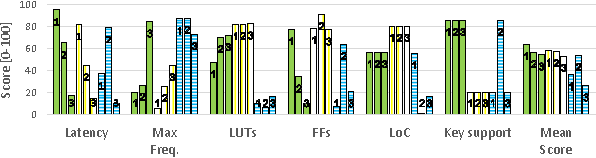
\includegraphics[height=3.8cm]{graphics/AES_Compare.pdf} 
    \captionof{figure}{AES cypher RTL designs score comparison (higher = better)}
    \label{fig:AES_Compare_Graph}
  \end{minipage}
\end{table*}

The Hsing core clearly has the best performance among the different designs (but the lowest score on LUTs utilization). The primary reason it achieved this is because it uses LUTs instead of BRAMs. This enables the synthesizer to optimize the AES SBox function, and even pipeline it. DFiant uses its \code{lookupTable} library function to implement SBox, and we have yet to enable such an option for DFiant. 

Although the DFiant-generated RTL performance is not optimal, it can still  be improved without modifying the DFiant AES code, if the DFiant compiler is optimized. Moreover, this code has an adaptive pipeline, while the RTL cores pipelines are fixed. The Vivado implementation enjoys the same advantages as DFiant, and has even less LoC. However, the Vivado code does not support all possible keys and its maximum performance is far from optimum (we did not attempt to improve the HLS pragma directives).

If we assume all metrics have the same weight, the mean score places the DFiant solutions at the top. It is difficult to determine what is truly the best solution, but DFiant clearly has the best potential for further improvement without any modification to the original code.

           
\subsection{Case Study: Double Precision FP Multiplier}
\begin{table*}[t!]
	\centering
	\setlength\tabcolsep{2pt}
	\scriptsize
	  \begin{minipage}[t][4.8cm][t]{0.8\linewidth}
	    \centering
	    \captionof{table}{FP Multiplication RTL Designs Comparison\\(the numbering on the left associates configurations with \fig{fig:FP_Compare_Graph})}
	    \label{tbl:FP_Compare_Table}
	    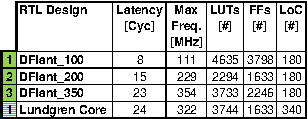
\includegraphics[scale=1.2]{graphics/FP_Compare_Table.pdf} 
	  \end{minipage}
    \\
	  \begin{minipage}[b][3.8cm][b]{\linewidth}
	    \centering
	    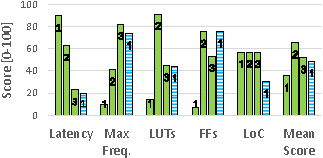
\includegraphics[height=3.8cm]{graphics/FP_Compare.pdf} 
	    \captionof{figure}{FP multiplication RTL designs score comparison (higher = better)}
	    \label{fig:FP_Compare_Graph}
	  \end{minipage}
\end{table*}

We compared our FP multiplier with the open IEEE-754 compatible Lundgren core \cite{lundgren2014open} (the only IEEE-754 fully compatible FP multiplication RTL design we had access to). Since the core is a complete floating point unit, we disabled the unnecessary parts, reducing it to only a FP multiplication, for a fair comparison with DFiant's code. The DFiant code was written by using the Lundgren VHDL code as a reference design. The designs are very similar in their structure, except that DFiant is considerably less verbose, and has no explicit pipeline.

We had no access to an open Vivado HLS FP multiplier for comparison. We could have directly invoked a \code{double} multiplication, but an inspection of the generated RTL revealed that Vivado HLS just instantiates an RTL floating point blackbox core. DFiant can choose to use this core as well, and achieve identical performance to Vivado HLS. Furthermore, the Vivado HLS floating point implementation is not fully compatible with IEEE-754 (e.g, does not support denormalized numbers).

Similarly to the AES case study, we collected the results in Table~\ref{tbl:FP_Compare_Table}, and displayed their normalized standard score in Fig.~\ref{fig:FP_Compare_Graph}. In comparison with the Lundgren core, DFiant\_350 is better in every criteria, aside from FFs utilization. Ultimately, DFiant out-performs its reference design for FP multiplication, and demonstrates its ability to provide different RTLs for design space exploration.

